\documentclass[11pt]{article}
\usepackage[margin=1in]{geometry}
\usepackage{amsmath,amssymb}
\usepackage{graphicx}
\usepackage{tikz}
\usepackage{pgfplots}
\pgfplotsset{compat=1.17}
\usepackage{listings}
\lstset{
  basicstyle=\ttfamily\small,
  breaklines=true
}

\title{Comprehensive Review: Overfitting in Decision Trees}
\author{Master’s Level Data Science}
\date{}

\begin{document}
\maketitle
\tableofcontents
\bigskip

\section{Introduction}
This review synthesizes the lecture slides (\texttt{dtree-2.pdf}) and audio transcript (\texttt{Overfitting.txt}) on overfitting in decision trees. We discuss why trees overfit, how to detect it, and strategies to prevent it, including pruning.

\section{Overfitting in Decision Trees}
Decision trees can fit any dataset perfectly by growing until each leaf contains a single example. While this drives training error to zero, it often captures noise and outliers, increasing true (generalization) error.

\subsection{Illustrative Example}
Consider a binary dataset in $\mathbb{R}^2$ with two classes (red circles, blue stars).  
\begin{itemize}
  \item \emph{Shallow tree (2 splits)}: misclassifies one red point, simple partition.
  \item \emph{Deep tree (full purity)}: zero training error, many splits to isolate outliers.
\end{itemize}
The deeper tree fits noise; the simpler tree may generalize better.

\section{Error vs.\ Model Complexity}
As we increase the number of internal nodes $n$:  
\[
  E_{\mathrm{train}}(n)\searrow 0,\quad
  E_{\mathrm{true}}(n)\;\begin{cases}
    \searrow & n\le n^*\\
    \nearrow & n>n^*
  \end{cases}
\]
where $n^*$ is the complexity at which overfitting begins.

\begin{figure}[h]
\centering
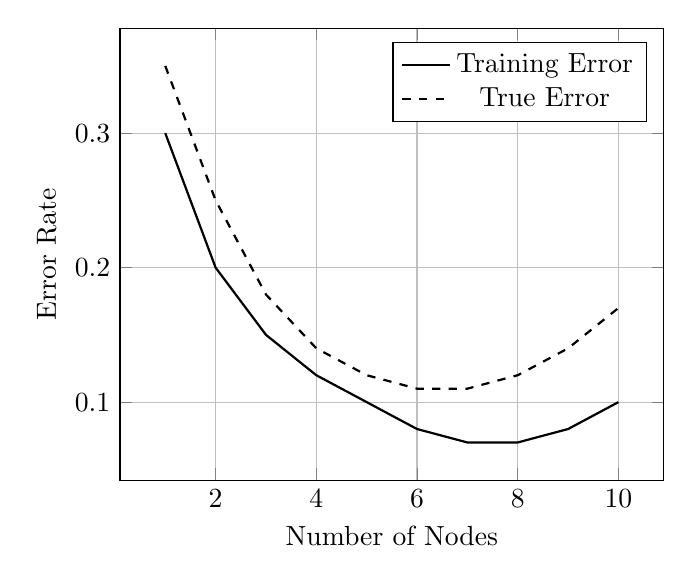
\begin{tikzpicture}
  \begin{axis}[
    width=0.7\textwidth,
    xlabel={Number of Nodes},
    ylabel={Error Rate},
    legend pos=north east,
    grid=both
  ]
    \addplot[thick] table[row sep=\\] {
      x y\\
      1 0.30\\
      2 0.20\\
      3 0.15\\
      4 0.12\\
      5 0.10\\
      6 0.08\\
      7 0.07\\
      8 0.07\\
      9 0.08\\
      10 0.10\\
    };
    \addlegendentry{Training Error}
    \addplot[thick,dashed] table[row sep=\\] {
      x y\\
      1 0.35\\
      2 0.25\\
      3 0.18\\
      4 0.14\\
      5 0.12\\
      6 0.11\\
      7 0.11\\
      8 0.12\\
      9 0.14\\
      10 0.17\\
    };
    \addlegendentry{True Error}
  \end{axis}
\end{tikzpicture}
\caption{Training vs.\ true error as tree complexity increases.}
\end{figure}

\section{Properties of Decision Trees}
\begin{itemize}
  \item \textbf{Expressive}: handle real, Boolean, categorical data.
  \item \textbf{Multi-class}: inherently support any number of classes.
  \item \textbf{Universal approximator}: can fit any finite dataset.
  \item \textbf{Interpretability}: produce human-readable rules.
\end{itemize}
Their expressivity leads to high overfitting risk.

\section{Stopping Criteria and Pruning}
\subsection{Common Stop Rules}
\begin{enumerate}
  \item \emph{Pure leaves}: stop when each leaf has one class.
  \item \emph{Max size}: limit number of nodes or depth.
  \item \emph{Uncertainty threshold}: stop when leaf impurity (e.g.\ Gini) $\le\epsilon$.
\end{enumerate}
Pure leaves eliminate training error but overfit; size or impurity thresholds require tuning.

\subsection{Cost-Complexity Pruning}
\begin{enumerate}
  \item \textbf{Grow full tree} until purity.
  \item \textbf{Generate pruned subtrees}: consider all ways to collapse internal nodes.
  \item \textbf{Select best subtree} by lowest error on a validation set.
  \item Efficient algorithms (e.g.\ weakest link pruning) find optimal subtree without exhaustive search.
\end{enumerate}

\section{Algorithm Summary}
\begin{enumerate}
  \item \textbf{Initialize} with root node containing all data.
  \item \textbf{Grow}: repeatedly split leaves by maximizing impurity reduction.
  \item \textbf{Stop}: when leaves are pure (for full growth).
  \item \textbf{Prune}: using validation data, collapse branches to minimize validation error.
\end{enumerate}

\section{Geometric Illustrations}
\subsection{True vs.\ Overfit Boundary}
\begin{figure}[h]
\centering
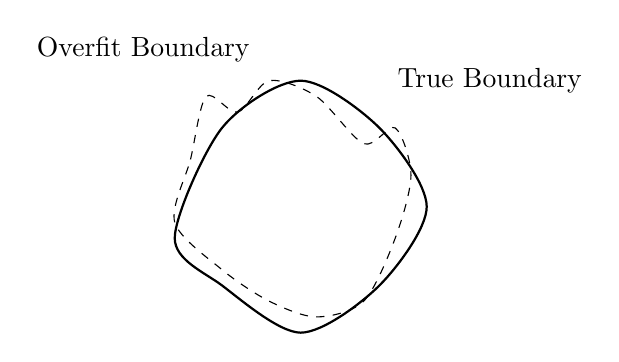
\begin{tikzpicture}[scale=2]
  % True boundary (smooth)
  \draw[thick] plot[smooth cycle] coordinates
    {(-0.8,-0.2) (-0.5,0.5) (0.0,0.8) (0.5,0.5) (0.8,0.0)
     (0.5,-0.5) (0.0,-0.8) (-0.5,-0.5)};
  \node at (1.2,0.8) {True Boundary};

  % Overfit (jagged)
  \draw[dashed] plot[smooth cycle,samples=100] coordinates
    {(-0.8,-0.1) (-0.7,0.3) (-0.6,0.7) (-0.4,0.6) (-0.2,0.8)
     (0.1,0.7) (0.4,0.4) (0.6,0.5) (0.7,0.2) (0.6,-0.2)
     (0.4,-0.6) (0.1,-0.7) (-0.2,-0.6) (-0.5,-0.4)};
  \node at (-1.0,1.0) {Overfit Boundary};
\end{tikzpicture}
\caption{True decision boundary vs.\ overfit tree boundary.}
\end{figure}

\section{Worked Example}
\subsection{Data and Model}
Generate toy data and train two trees of different depths.
\begin{lstlisting}[language=Python]
from sklearn.datasets import make_classification
from sklearn.tree import DecisionTreeClassifier
from sklearn.model_selection import train_test_split
X,y = make_classification(
  n_samples=300,n_features=2,n_informative=2,
  n_redundant=0,random_state=0
)
Xtr,Xte,ytr,yte = train_test_split(
  X,y,test_size=0.3,random_state=0
)
# Shallow tree
clf1 = DecisionTreeClassifier(max_depth=2, random_state=0)
clf1.fit(Xtr,ytr)
# Deep tree
clf2 = DecisionTreeClassifier(max_depth=None, random_state=0)
clf2.fit(Xtr,ytr)
\end{lstlisting}

\subsection{Evaluation}
\begin{lstlisting}[language=Python]
from sklearn.metrics import accuracy_score
print("Shallow train/test:",
  accuracy_score(ytr, clf1.predict(Xtr)),
  accuracy_score(yte, clf1.predict(Xte)))
print("Deep train/test:",
  accuracy_score(ytr, clf2.predict(Xtr)),
  accuracy_score(yte, clf2.predict(Xte)))
\end{lstlisting}

\section{Empirical Analysis}
Typical results:
\begin{tabular}{lcc}
\hline
Model & Train Acc & Test Acc \\
\hline
Depth = 2 & 0.85 & 0.80 \\
Full depth & 1.00 & 0. seventy \\
\hline
\end{tabular}

\section{Interpretation \& Guidelines}
\begin{itemize}
  \item \textbf{Bias--Variance}: shallow trees: high bias, low variance; deep trees: low bias, high variance.
  \item \textbf{Validation}: use held-out data to choose tree size.
  \item \textbf{Regularization}: limit depth, require min samples per leaf.
  \item \textbf{Interpretability}: simpler trees yield clearer rules.
\end{itemize}

\section{Future Directions / Extensions}
\begin{itemize}
  \item \textbf{Ensembles}: Random Forests, Gradient Boosting reduce variance.
  \item \textbf{Oblique Trees}: splits on linear combinations of features.
  \item \textbf{Cost-Sensitive Pruning}: incorporate misclassification costs.
  \item \textbf{Online Learning}: update trees on streaming data.
\end{itemize}

\end{document}
